\documentclass{article}

\usepackage{graphicx}
\usepackage{hyperref}
\usepackage{geometry}
\usepackage{amsmath}
\title{An Analysis on Chronic Kidney Disease Public Health Data}
\author{Akshay Sanjeev}
\date{\today}

\begin{document}
\maketitle

\section*{Preface}
\subsection{Notation and Convention}
By standard dataset, from now on I will be referring to the following data structure. 
We have $m$ independent variables(a.k.a features), denoted by $x^i, i = 1,2,3, \cdots,m$ 
and one dependent variable(a.k.a label), $m$. Let $n$ be the total number of observations, 
and the lower index denotes the observation. Thus the dataset is set like the one given below. 
\begin{equation}
    \begin{pmatrix}
        x^1_1 & x^2_1 & \cdots & x^m_1 & y_1 \\
        x^1_2 & x^2_2 & \cdots & x^m_2 & y_2 \\
        \vdots & \vdots & \ddots & \vdots & \vdots \\
        x^1_n & x^2_n & \cdots & x^m_n & y_n
    \end{pmatrix}
\end{equation}

\subsection{Model Evaluation}

\begin{center}
\begin{tabular}{|c|c|c|}
\hline
 & \textbf{Predicted Positive} & \textbf{Predicted Negative} \\
\hline
\textbf{Actual Positive} & $TP$ (True Positive) & $FN$ (False Negative) \\
\hline
\textbf{Actual Negative} & $FP$ (False Positive) & $TN$ (True Negative) \\
\hline
\end{tabular}
\end{center}

\subsubsection*{Accuracy}
Accuracy is the proportion of all predictions (both positive and negative) that were correct. It is not recommended when dealing with imbalanced datasets.
\[
\text{Accuracy} = \frac{TP + TN}{TP + TN + FP + FN}
\]

\subsubsection*{Recall(TPR)}
Also known as the true positive rate or sensitivity, recall measures the proportion of actual positive cases that were correctly identified.
\[
\text{Recall} = \frac{TP}{TP + FN}
\]

\subsubsection*{False Positive Rate (FPR)}
The false positive rate measures the proportion of actual negatives that were incorrectly classified as positive. Ideally, this should be close to zero.
\[
\text{FPR} = \frac{FP}{FP + TN}
\]

\subsubsection*{Precision}
Precision is the proportion of predicted positive cases that are truly positive.
\[
\text{Precision} = \frac{TP}{TP + FP}
\]

\subsubsection{ROC curve}
ROC curve is plotted as true positive rate(TPR) on $y$ axis and false positive rate(FPR) on $x$ axis. Ideally
we want TPR to be 1 and FPR to be 0. Hence the closer it follows the left and upper axis, better
the results. Another related measure is the area under the ROC curve. The best result would be AuC = 1. 




\section{Pre-Processing Data and Question}
The motivation to pre- process data is that you need the dataset in a 
machine readable format. The raw dataset, titled \texttt{CKD\_agri\_data.xls} is in the 
following format. 3350 rows correspond to individuals and 151 columns contain
various information about these individuals. The columns have various information It has
metadata like name, age, sex and so on, medical information, disease history, test reports and etc. 
This is a mix of numeric and categoric variables. 

The first issue I found was the missing observations. I looked at the what fraction of data is missing for 
each row and column and  plotted the sorted fraction in figure \ref{fig:thresholding}. I set thresholds
for the both row-wise and column-wise fraction and only kept the observations below the threshold. The blue 
line in figure \ref{fig:thresholding} represents the threshold in both cases. 
\begin{figure}
    \centering
    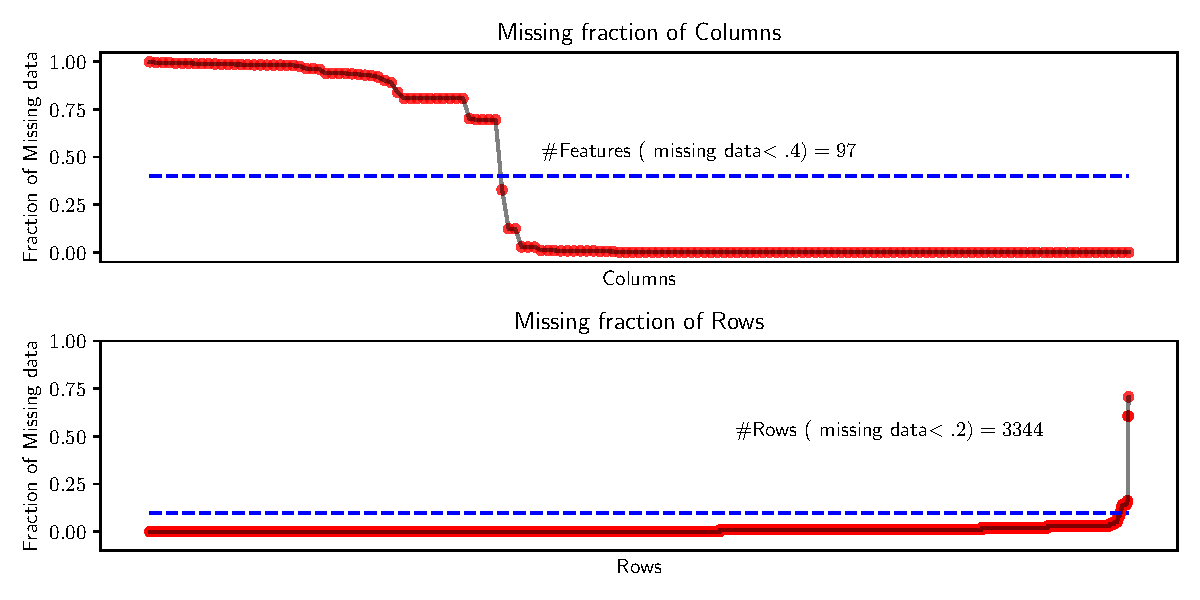
\includegraphics[width=\textwidth]{pp_frac.pdf}
    \caption{Fraction of missing data corresponding to each column(Top) and each row(Bottom).}
    \label{fig:thresholding}
\end{figure}

Second issue was that some features had erroneous feature names and values. I corrected the feature 
names and replaced the erroneous values with the median of the respective feature. At this point, 
the dataset was mostly clean and ready for further analysis. For categorical variables with erroneous
or missing values, I replaced them with the mode (most frequent value) of the respective feature.


I had 46 numeric features and 54 categoric features now. To begin the analysis I only chose the 
numeric features and created the dataset. Among the numeric dataset, I had four features related to Chronic
Kidney Disease(\texttt{ckd\_final, ckd\_epi\_sample\_1,ckd\_\_probable\_sample\_1, ckd\_code\_sample\_1 }). 
\begin{figure}
    \centering
    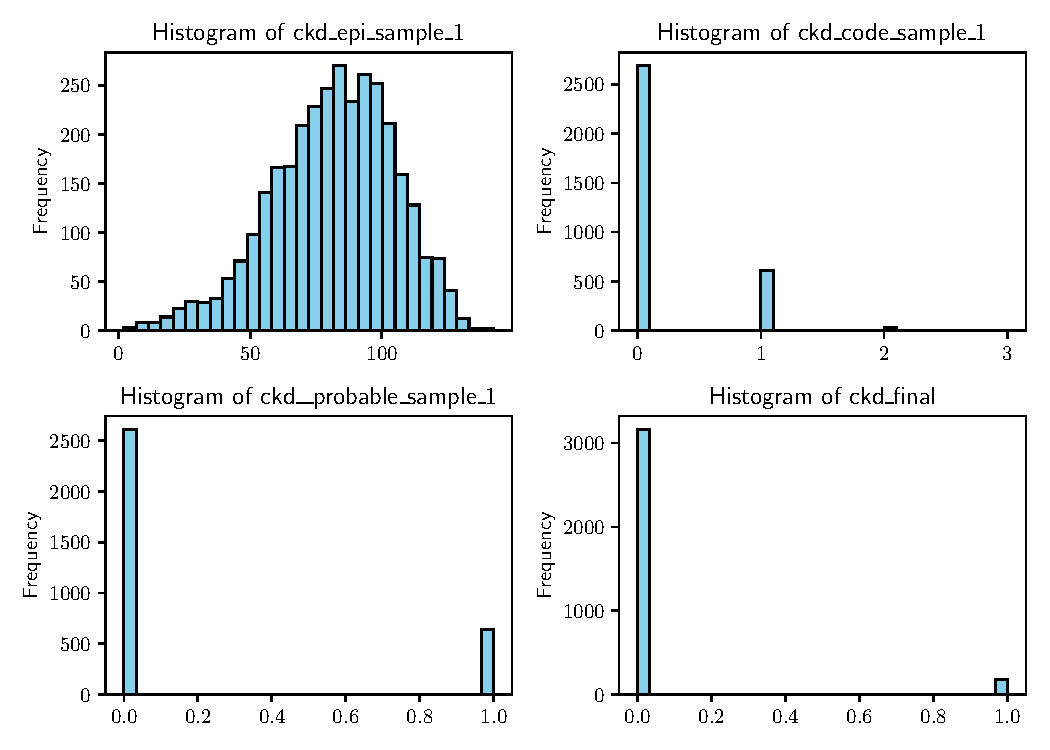
\includegraphics[scale=.7]{4var_hist.pdf}
    \caption{Distribution of potential target variables}
    \label{fig:4varhist}
\end{figure}

But since the only information I have is the feature name, it is hard to predict what they mean.
But looking at the unique values in each column, I inferred that \texttt{ckd\_final} and 
\texttt{,ckd\_\_probable\_sample\_1} are binary variables and \texttt{ckd\_\_probable\_sample\_1} has 0, 1, 2
and 3 as unique values and the last one is roughly in the range 0-145. The histogram of these four variables 
are given in figure \ref{fig:4varhist}.

\subsection{Question}
Since the dataset primarily target on chronic Kidney disease, the first question we are intersted in is
given the numeric data collected, can we use machine learning based methods to predict whether a 
person having chronic kidney disease or not. 
\begin{figure}
    \centering
    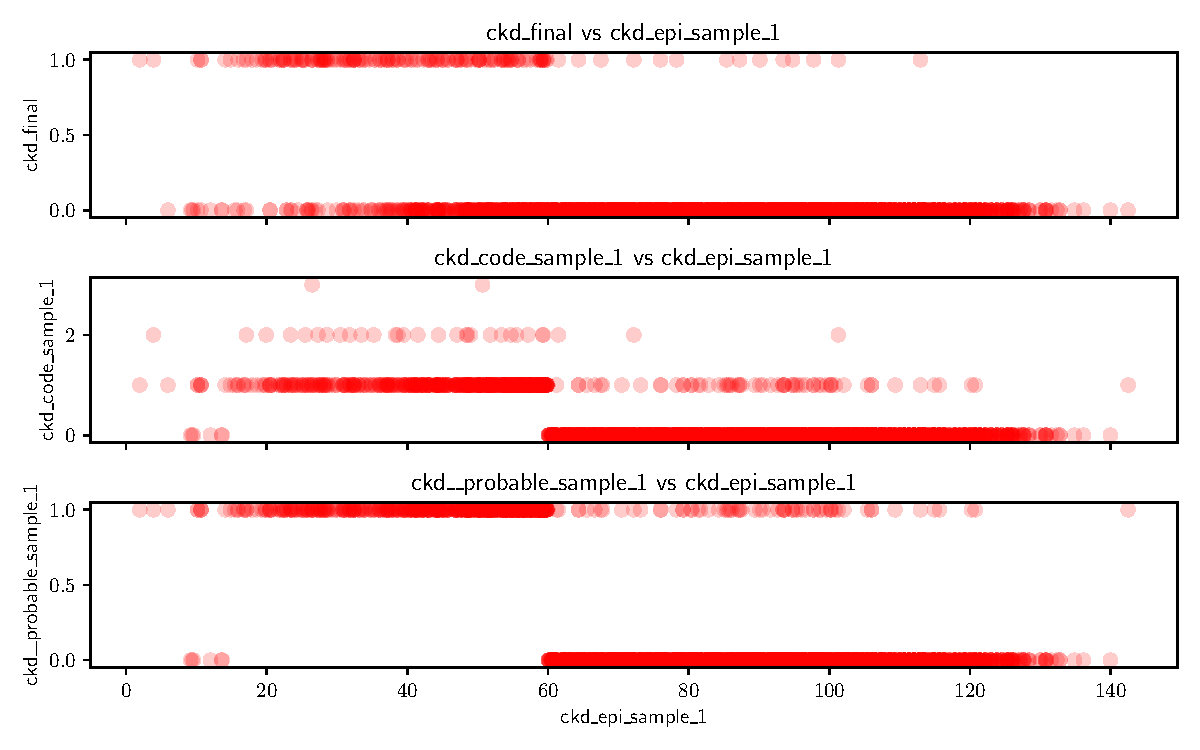
\includegraphics[scale=.7]{targetvar_correlation.pdf}
    \label{fig:4varcorr}
    \caption{Each subplot is trying to visualise relation between target variable, \texttt{ckd\_code\_sample\_1}
    with other 3 variables related to chronic Kidney disease. }
\end{figure}
I tried to find a correlation between the numeric CKD feature and other features in pursuit of picking 
a target variable among the four. The plots are in figure \ref{fig:4varcorr}. Qualitatively, \texttt{ckd\_\_probable\_sample\_1} has the highest correlation. But 
I think it's okay to remove all four from training data to be safe. For the target variable, I choose 
\texttt{ckd\_code\_sample\_1}. Presumably, the variable has the optimal information, because it predicts
3 stages of chronic Kidney disease.\par 
Now that the question is clear, we will use Decision Trees, Random Forest and Feed-froward Neural Network models 
on the data. 


\section{Decision Tree}
\subsection{Informal Description(DT)}
A decision tree is a supervised learning method, where you split data based 
on a nested \texttt{if} and \texttt{else} conditions. To build a decision tree, 
\begin{enumerate}
    \item take the standard dataset, compute the Shannon Entropy for each variable 
        \[H^i = -\sum_j^n p(x^i_j)\log p(x^i_j)\]
    \item Classify or predict the dependent variable based on those each variable and compute 
    the Information Gain($IG^i$) for each variable,
    \[ IG^i = H^i - \sum_s \frac{|x^{is}|}{|x^{i}|} H^is \], where $x^{is}$ is the set of
    $s$-th split of dataset. 
    \item Pick the feature with maximum $IG$ and assign that for the node. 
    \[x_{\text{selected}} = \arg \max_{i} (IG^i)\]
\end{enumerate}
Repeat the step one to three iteratively by moving down the tree,as you pick a feature and 
assign it to a node, until all nodes become terminal. A node is terminated if the it has an 
zero entropy. 

\subsubsection{Sensitivity}
This is a greedy splitting. At each step the aim is to make immediate improvements, which may 
not be the best at  a global level. It is a local phenomenon. Also if we don't set a maximum 
depth, trees grow deeper and may end up in memoriing the training data and over-fitting. This 
overall results in poor generalisation and high variance. This can be tackled with a couple of 
methods(pruning, specified tree depth and minimum samples per terminal node, ensemble of trees 
etc.)

\subsection{Results}
% \begin{figure}
%     \centering
%     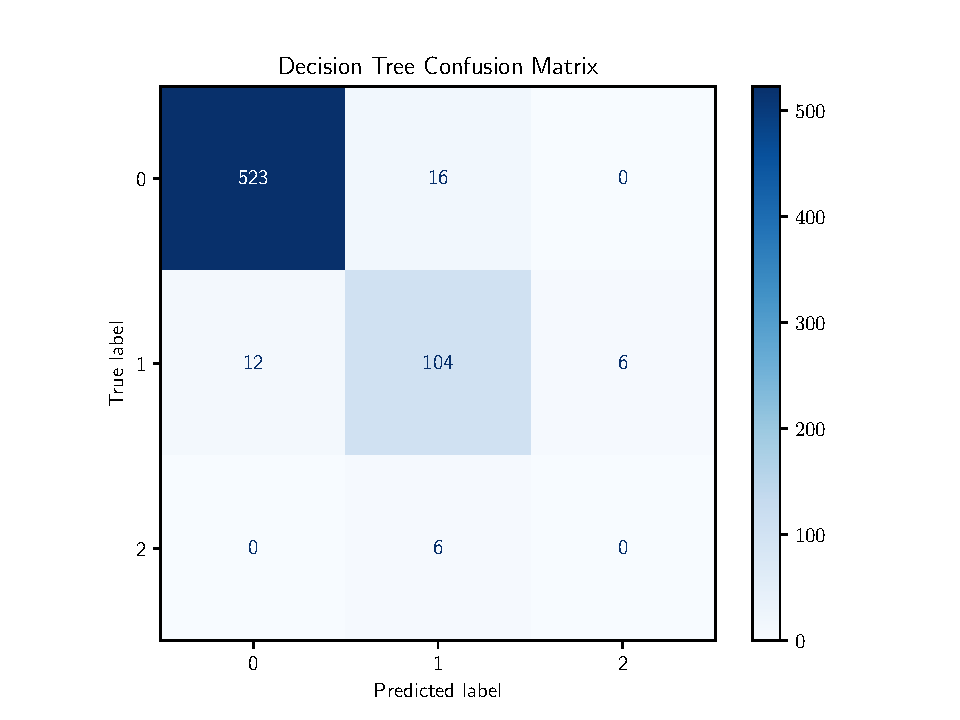
\includegraphics[scale=.5]{DT_conf_matrix.pdf}
%     \label{fig:DT_cmat}
%     \caption{Confusion matrix of Decision tree classification. Precisions values are 
%     0.98, 0.83 and 0 for class 0, 1 and 2 respectively. Accuracy is 0.94}
% \end{figure}
\begin{figure}
    \centering
    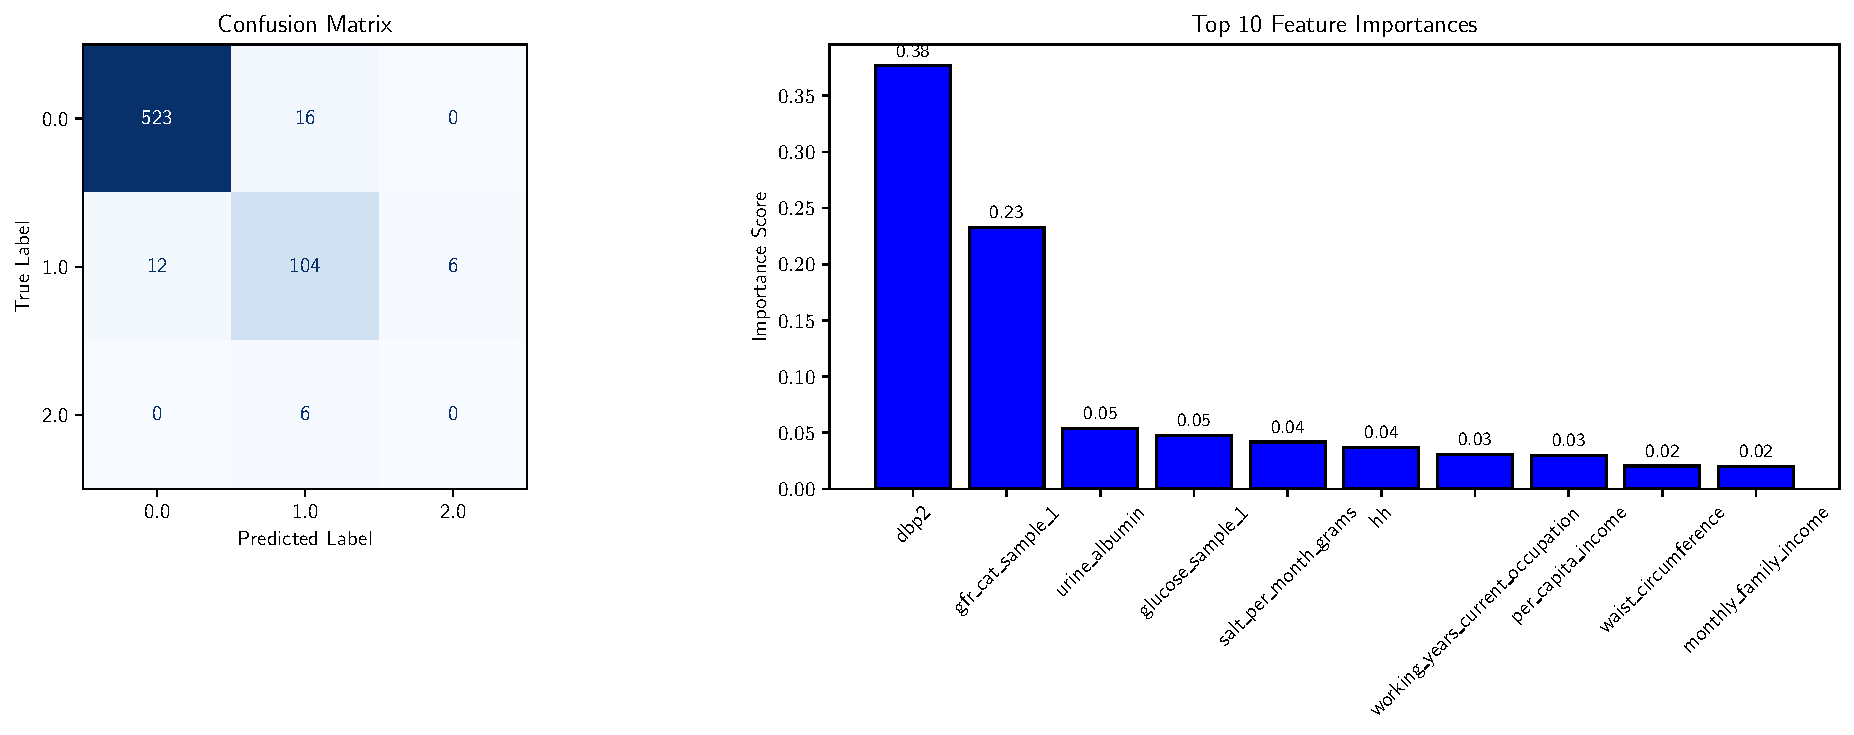
\includegraphics[scale=.5]{DT_summary.pdf}
    \label{fig:DTsum}
    \caption{(Left) Confusion matrix of Decision tree classification. Precisions values are 
    0.98, 0.83 and 0 for class 0, 1 and 2 respectively. Accuracy is 0.94, (Right) The 10 highest contributing features
    to the model.}
\end{figure}
I build a decision tree and carried out the analysis using Python 3.11 and \href{https://scihttps://scikit-learn.org/}{scikit-learn}
a machine learning package in Python. The tree was built using the Entropy criterion and 
the rest of the parameters are kept default. The classification results are represented as a 
confusion matrix in figure \ref{fig:DTsum}. The classifier did a very good job for class 0 and 1. But possibly due
to the scarcity in training data, the the class 2 didn't perform well. Class 3 was too rare, 
that it was not present in testing data. 

The contribution of each feature in figure \ref{fig:DTsum}. The highest contributing features are \texttt{dbp2} and 
\texttt{gft\_cat\_sample\_1}.
To conclude from public health data we can infer potential chronic Kidney disease patients,
given it contains reliable medical test information, as we have seen above 
test results like \texttt{dbp2} and \texttt{gft\_cat\_sample\_1} are the most important features. 
Qualitatively all other features seems to contribute very minimally. But some statistical significance measure is 
recommended for a reliable conclusion. 


\section{Random Forest(RF)}
\subsection{Informal Description}
Random Forest is an ensemble of Decision Trees. The justification for building an ensemble 
of Decision Trees is to reduce variance and sensitivity. To be specific, it uses a method called
Bootstrap Aggregation. First sample various sets of  observations and features with replacement from the    
independent decision trees. The final prediction is done by using averaging or major-voting depending 
on the varibale.  For example we have a model,  $\hat{f}^i(x),(i = 1,2,3, \cdots, B)$ and $B$ bootstrapped 
datasets and our final prediction for a regression will be
\[
\hat{f}_{\text{avg}}(x) = \frac{1}{B}\sum_{i=1}^B \hat{f}^i(x)
\]. 

\subsection{Analysis \& Results}
\begin{figure}
    \centering
    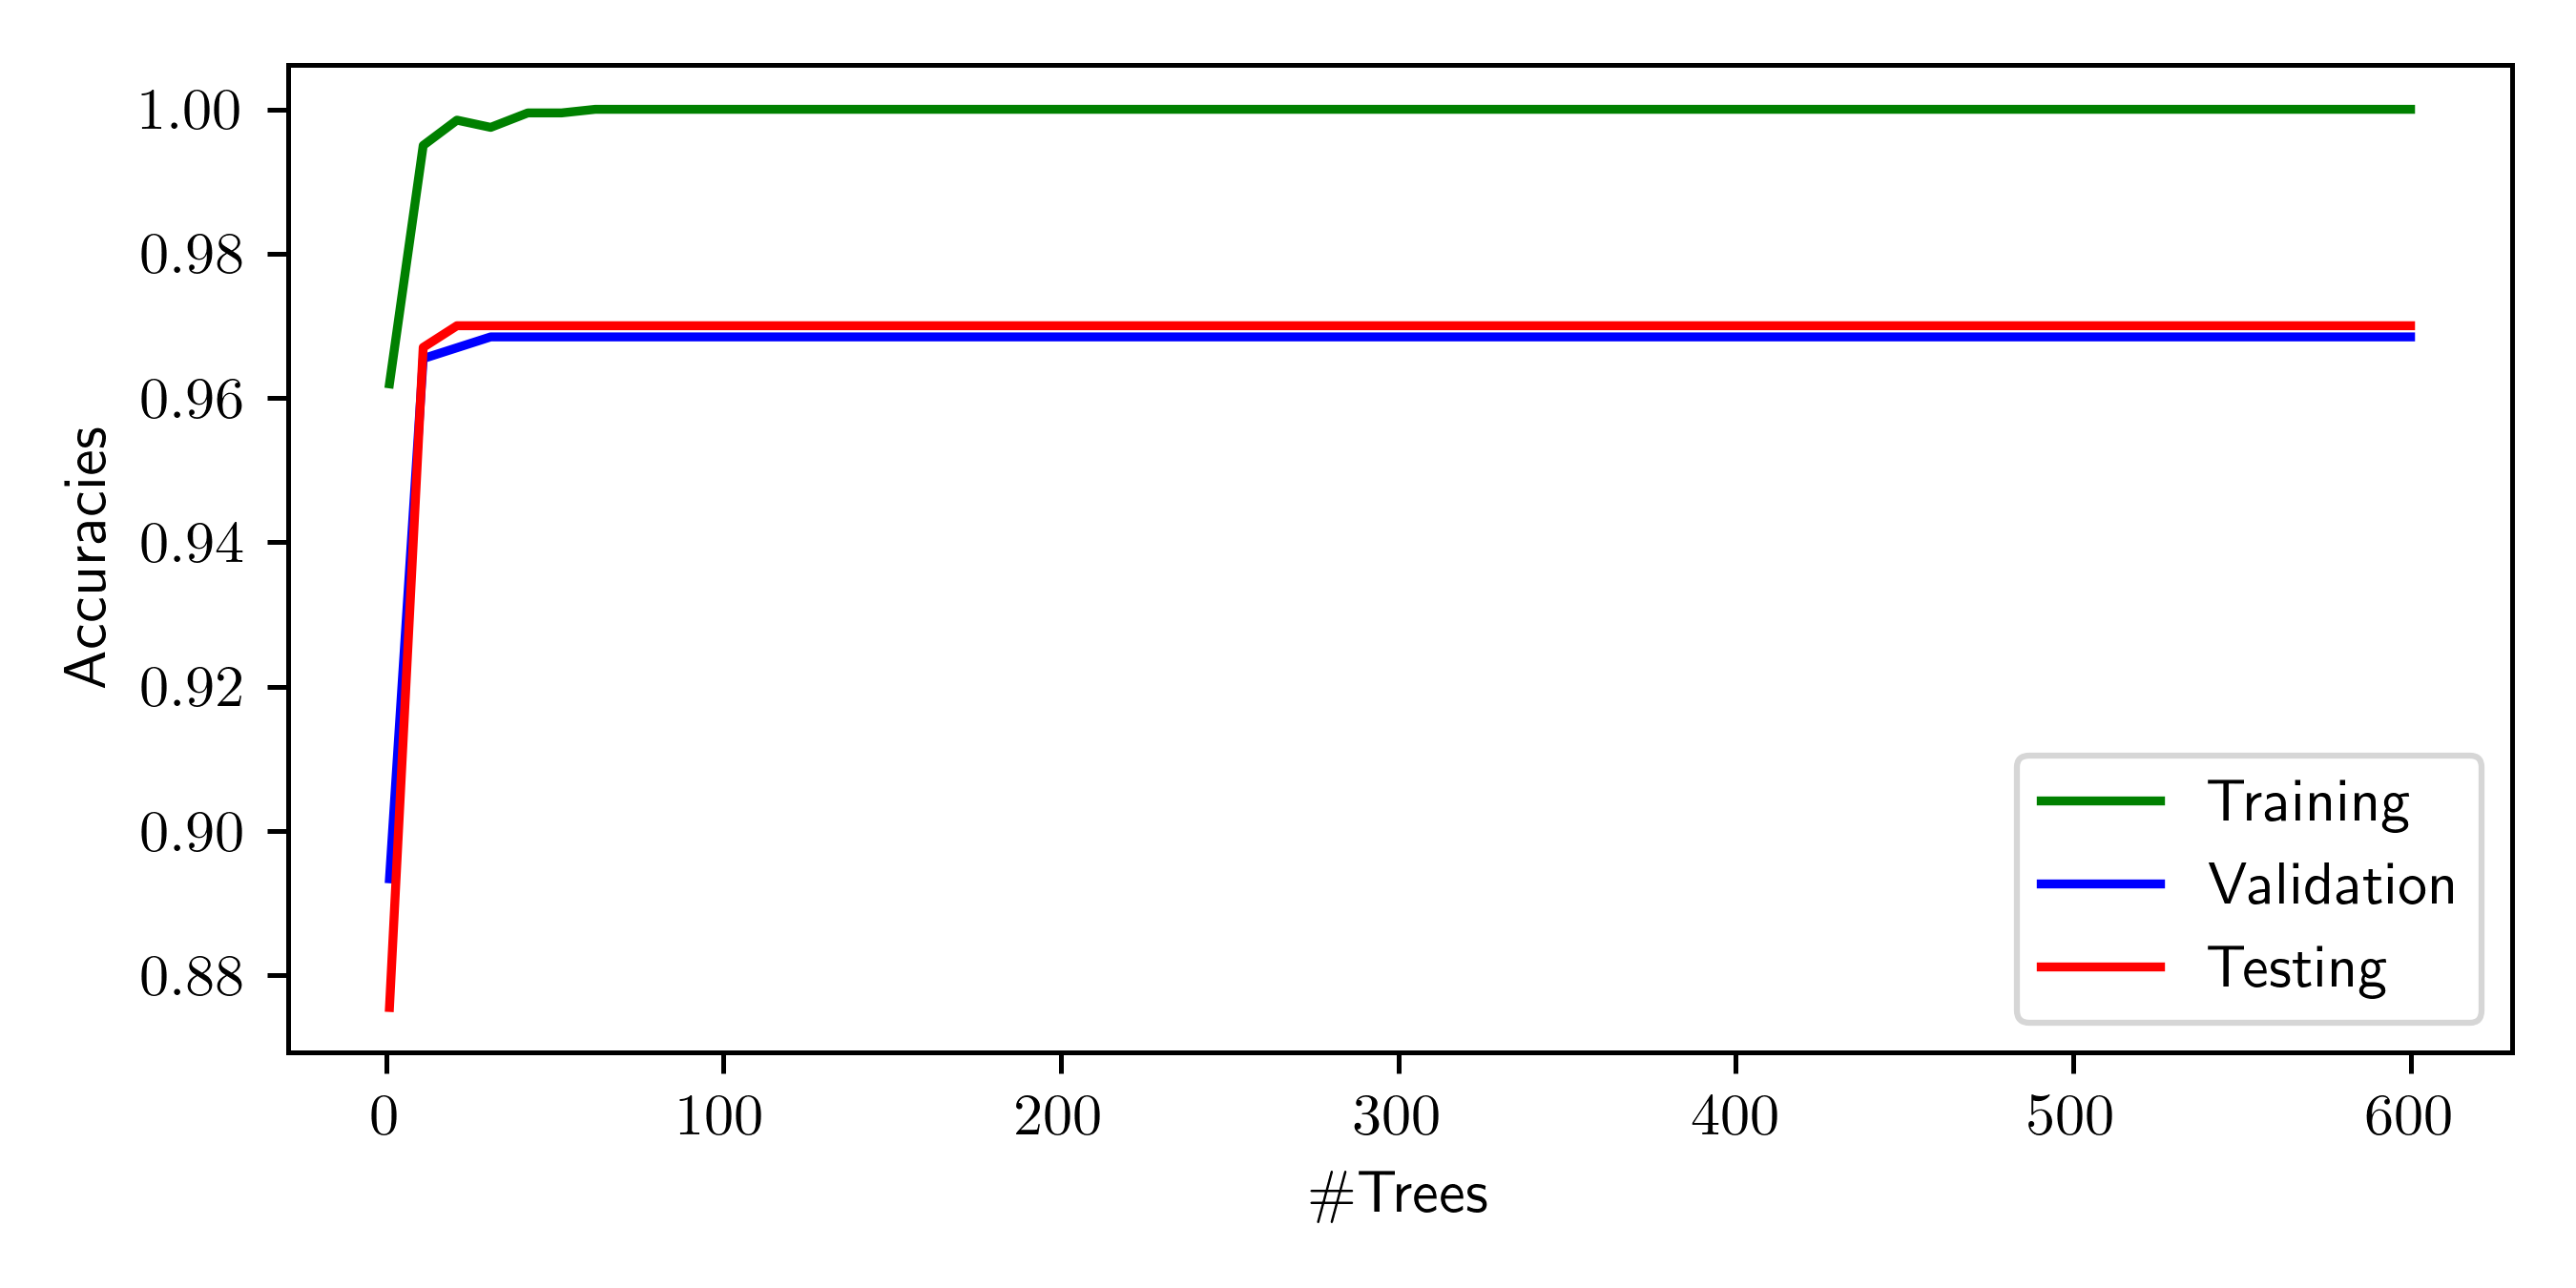
\includegraphics[scale=.75]{RF_acc_tree.png}
    \label{fig:treeacc}
    \caption{}
\end{figure}
Similar to the above case, I have used Python 3.11 and \href{https://scihttps://scikit-learn.org/}{scikit-learn}
to build Random Forest, classify and analyse the results. Rather jumping into the classification problem we have, 
at first I was interested in is how would the algorithm perform as you increase the number of trees. So I computed 
the accuracy of random forest, with 1 to 600 trees(figure \ref{fig:treeacc}). The accuracy of classification saturates
for both training and validation dataset a little early than 100 trees. Thus I picked 100 trees and did the classification. 

The summary of a result with confusion matrix and feature importance are plotted in \ref{fig:rfsum}. As we have seen for 
Decision tree, class 0 and 1 are fairly good. Now class 2 also doesn't have any observations in testing data. We can see 
a much wider feature importance here. Interestingly the highest contributing feature earlier is shifted to third place. 
The importance of leading features have also lowered, implying a more balanced classification.  

\begin{figure}\centering
    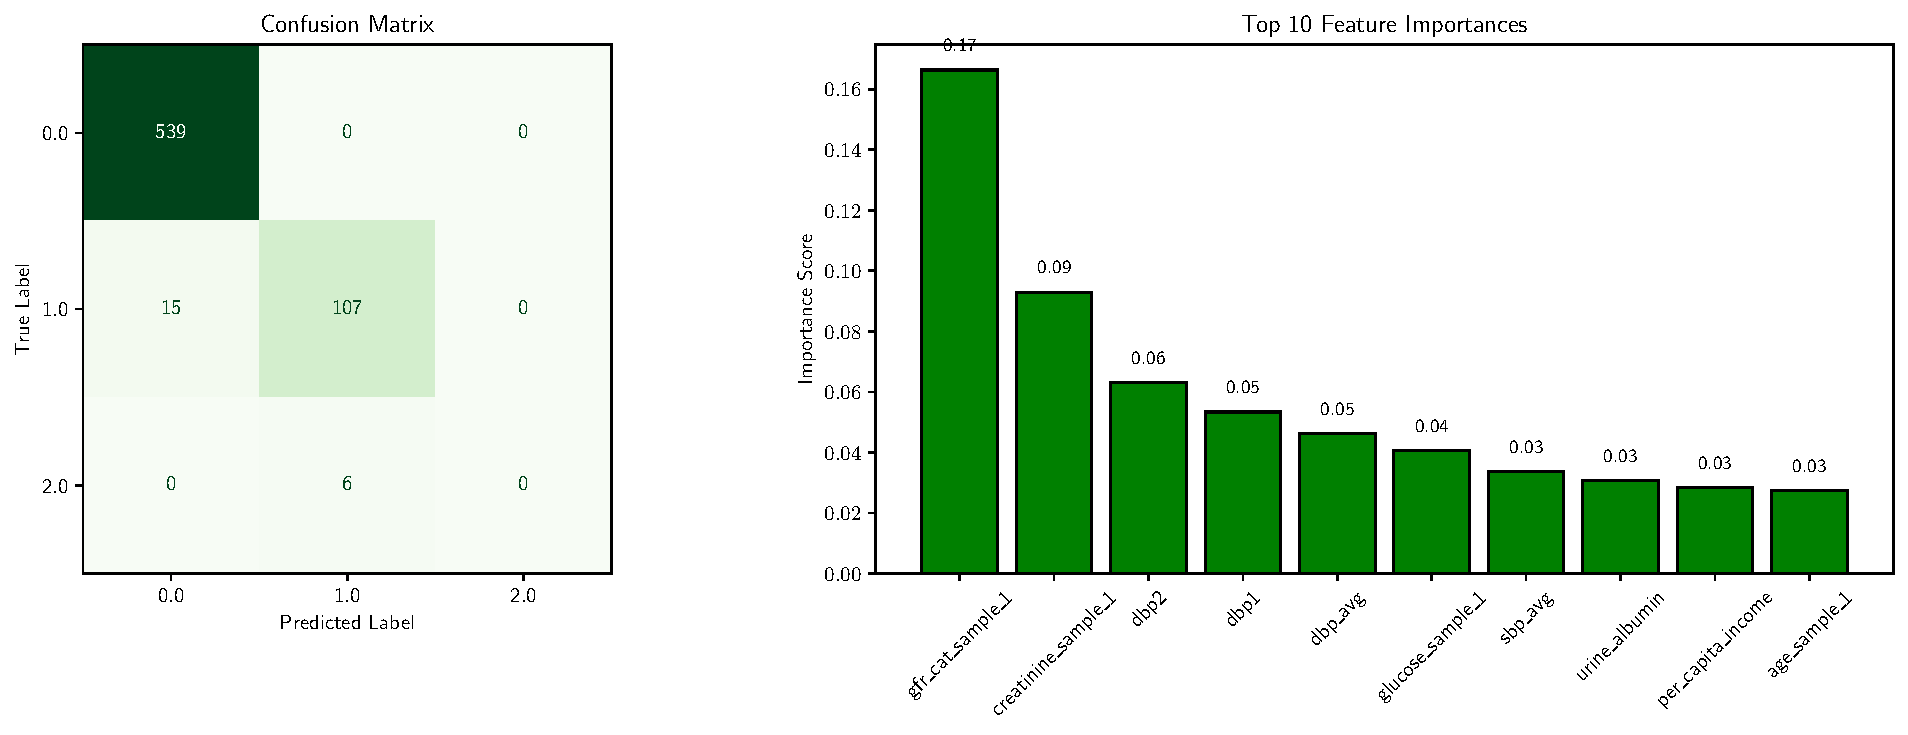
\includegraphics[scale=.75]{RF_summary.pdf}
    \label{fig:rfsum}
    \caption{(Top, Left) Confusion matrix of Random Forest classification. Precisions values are 
    0.97, 0.95 and 0 for class 0, 1 and 2 respectively. Accuracy is 0.97, (Top, Right) ROC curve for different
    classes. (Bottom) The 10 highest contributing features
    to the model.}
\end{figure}
From the ROC curve in the figure \ref{fig:rfsum} also implies a fair classification for 
class 0 and 1. Eventhough no class 2 observations were predicted correctly, class 2 having 
a high area under the ROC curve(0.9284) is hard to understand. 

To recapitulate, switching from decision tree to random forest, had given us marginal increase
in accuracy. But I think the ensemble effect can be seen when we have large data to test the model on. 


\section{Feed-forward Neural Network(FFNL)}
\subsection{Informal Description}
Feed-forward Neural Network is a supervised machine learning algorithm, based on a a network of neurons 
or perceptron to be specific.  Each neuron behaves like a switch, depending on the inputs signals the neuron decides to 
turn ON or oFF, by plugging the inputs to an activation function. The network architecture is layered as shown in the figure \ref{fig:ffnl}.
Information flows from layer to layer, but not between nodes in the same layer. 
\begin{figure}
    \centering
    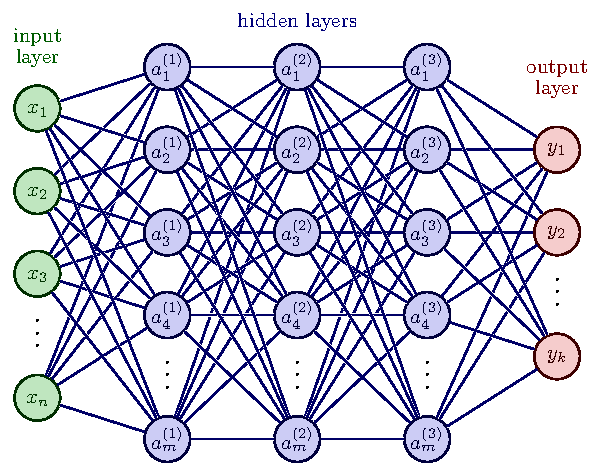
\includegraphics[scale=1]{ffnl.pdf}
    \caption{Schematic for a neural network}
    \label{fig:ffnl}
\end{figure}

For the $i$-th neuron on $l$-th layer, you get information from $l-1$ th layer and your input to this neuron $z^(l)_i$ is,
\[z^{(l)}_i = W^{(l)}_{ij}a_j^{(l-1)}+b^{(l)}_i\] 
where $W^{(l)}_{ij}$ is the weight of the matrix that goes from $j$ to $i$, $a_j^{(l-1)}$ is the output of $j$-th neuron in the 
previous layer. This input is plugged into an activation function, to compute the output of the neuron.
\[a^{(l)}_i = f^{(l)}_i(z^{(l)}_i)\].
The popular choices for activation function are ReLU, sigmoidal, Softamx, etc.,
We initiate and train the network with small random weights and make a prediction. Then compute how far is the prediction from the 
desired output, using a cost function. The next step is to minimize the cost, by tuning the set of parameters, $\theta$. You tune the parameters
along the negative cost gradient with a learning rate,$\epsilon$. The parameter set for the next prediction is,
\[\theta_{t+1} = \theta_t - \epsilon \frac{\partial}{\partial p} C(y, \hat{y})\] 
The cost gradient is estimated using chain rule. For the weight matrix, it can be written as:
\begin{align}
\frac{\partial C}{\partial W_{ij}} &= \frac{\partial C}{\partial a^L_i}\cdot \frac{\partial a^L_i}{\partial z^L_i}\cdot  \frac{\partial z^L_i}{\partial W_{ij}}\\
    & = \frac{\partial C}{\partial a^L_i}\cdot f^{(l)'}(z^{(l)}_i) \cdot a^{(l-1)}_j
\end{align}
You iteratively do this until you reach the minimum cost possible.The prediction part where you move from input to output is called forward propagation 
and the parameter tuning part is called back propagation. 

\subsection{Analysis \& Results}
Using \href{https://www.tensorflow.org/api_docs/python/tf/all_symbols}{ TensorFlow 2} in Pyhton 3.11. At first, I 
built an FFNL with 1 input layer with 46 input layers(same as the number of features),
one hidden layer with 32 neurons and the output layer with 4 neurons, because I have 
4 class labels. For the first two layers, I have a sigmoid activation function and
for the final layer I have softmax. I am training the network for 50 epochs. I have 
tried longer epochs, but the accuracy is saturated around 0.8, whihc doesn't look that bad.
But the classification matrix had the real horror. In figure \label{fig:ffnlsums}
you can see that everything was predicted as class 0 and since all class 0,  which 
dominated the training dataset, has been classified correctly the resulting accuracy
was 0.81. 
I made a bigger network,  with (45, 128, 64, 32, 4) and still the same. I varied the 
learning rate, $\epsilon$ and nothing changed. An interesting observation was the 
network is not learning. The \texttt{loss, va\_accuracy} and \texttt{val\_loss} are not 
changing at all and \texttt{accuracy} is fluctuating around 0.8. 
\begin{figure}
    \centering
    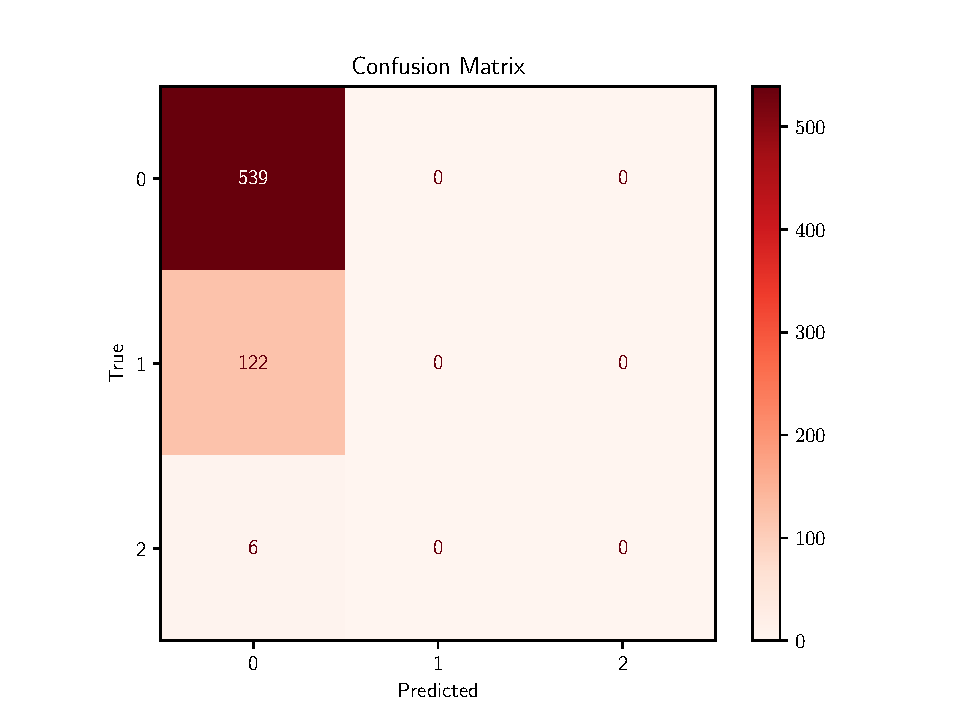
\includegraphics[scale=.5]{FFNL_summary.pdf}
    \caption{Confusion matrix for Feed-forward Neural Network. Precision of
    class 0, 1 and 2 are 0.81, 0 and 0 respectively. }
    \label{fig:ffnlsum}
\end{figure}

To conclude, I couldn't optimise the Feedforward neural network model for this problem. 


\end{document}